\documentclass[12pt]{amsart}
\usepackage{../marktext} 
%% Remove draft for real article, put twocolumn for two columns
\usepackage{../svmacro}
\usepackage[utf8]{inputenc}
\usepackage{lineno}
%\usepackage{authblk}
\usepackage[style=alphabetic, backend=biber]{biblatex}
\usepackage{enumitem}

%% commentary bubble
\newcommand{\SV}[2][]{\sidenote[colback=green!10]{\textbf{SV\xspace #1:} #2}}

%% Title 
\title{ MATH 170: Homework 8 }
%\author[1]{Co-author}
\author{Due: Nov 19, 2021}
%\affil[1]{Institute}
\date{}

\begin{document}

\maketitle


\noindent{\bf Graded for accuracy:}
1, 2.
\\
\noindent{\bf Graded for completion:}
3.
\\
\noindent{\bf Instructions:}
Problems that are graded for accuracy must be correct to get points.
Problems that are graded for completion must show some trying effort.

\centerline

\hrule

\centerline

\begin{enumerate}[label=\arabic*.,itemsep=10pt, leftmargin=*]


    \item 
    Let $A_k$ be the graph with $k$ vertices that looks like a line with marked points. Recall that $P_{A_k}(n)$ is the number of colorings of the vertices of $A_k$ into $n$ colors such that no two vertices that share an edge have the same color.
    
    \begin{center}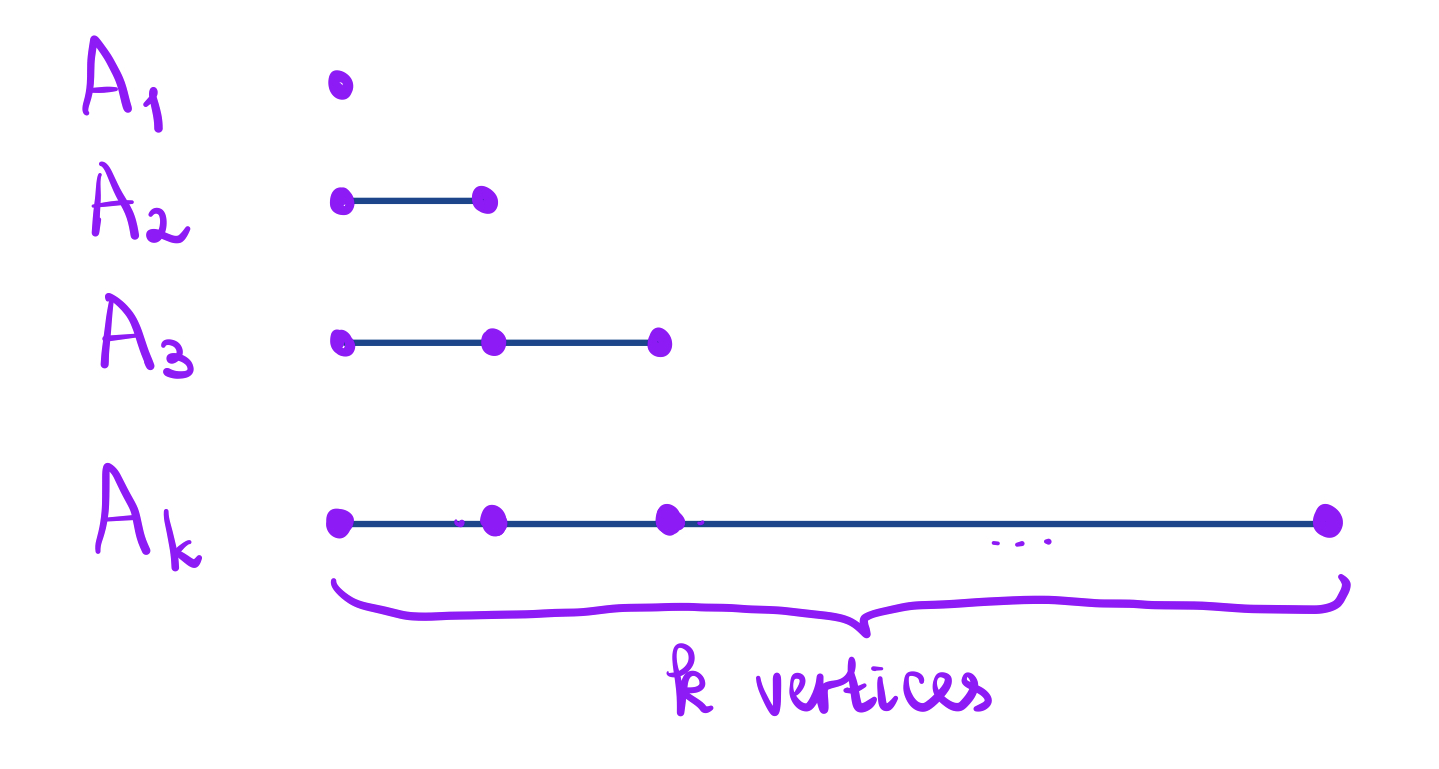
\includegraphics[width=8cm]{IMG_7164.jpg}\end{center}
    \begin{enumerate}
        \item
        Compute $P_{A_1}(3)$, $P_{A_2}(3)$, $P_{A_3}(3)$.
        
        \item 
        Guess the formula for $P_{A_k}(3)$ and prove it by induction.

        \end{enumerate}
        
    \item 
    Let $G$ be the following graph with 4 vertices and 6 edges.
    
    \begin{center}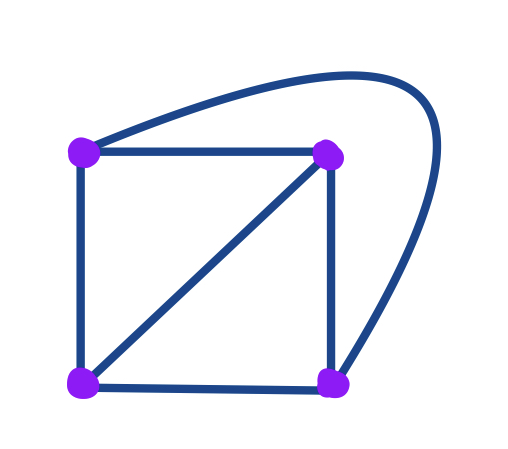
\includegraphics[width=5cm]{IMG_7165.jpg}\end{center}
    \begin{enumerate}
        \item 
        Compute $P_G(n)$ using the contraction-deletion formula.
        \item
        Using the previos part, compute the number of colorings of $G$ into 6 colors. (You may use a calculator.)
        \end{enumerate}

    
\item Set a timer and play Planarity (\url{https://www.jasondavies.com/planarity/}) for at least 10 minutes with 8 vertices. The game will show you how much time each round of untangling takes. Write your record time.
\end{enumerate}



\end{document}
